\documentclass{article}
\usepackage[T1]{fontenc}
\usepackage{lmodern}
\usepackage{graphicx}
\usepackage{amsmath,amssymb}
\usepackage[a4paper,margin=2cm]{geometry}
\usepackage[absolute,overlay]{textpos}
\setlength{\TPHorizModule}{1mm}
\setlength{\TPVertModule}{1mm}
\usepackage[indonesian]{babel}
\usepackage{hyperref}
\setlength{\emergencystretch}{2em}
% unit: Halaman 61

\begin{document}

% === Halaman 61 (llm) ===

\vspace{210.87mm}

\textbf{Plaintext input}
\vspace{50mm}
\textbf{Public key} \quad \textbf{Different keys} \quad \textbf{Private key}
\vspace{20mm}
\textcolor{red}{Sumber: Cryptography in E-Commerce}

% deskripsi: Diagram alur enkripsi dan dekripsi asimetris yang menunjukkan proses perubahan plaintext input menjadi ciphertext menggunakan public key, dan pengembalian ciphertext menjadi plaintext output menggunakan private key.
% bbox normalisasi: [0.1200, 0.1500, 0.8300, 0.8600]
\begin{textblock*}{149.10mm}(25.20mm,44.55mm)
\noindent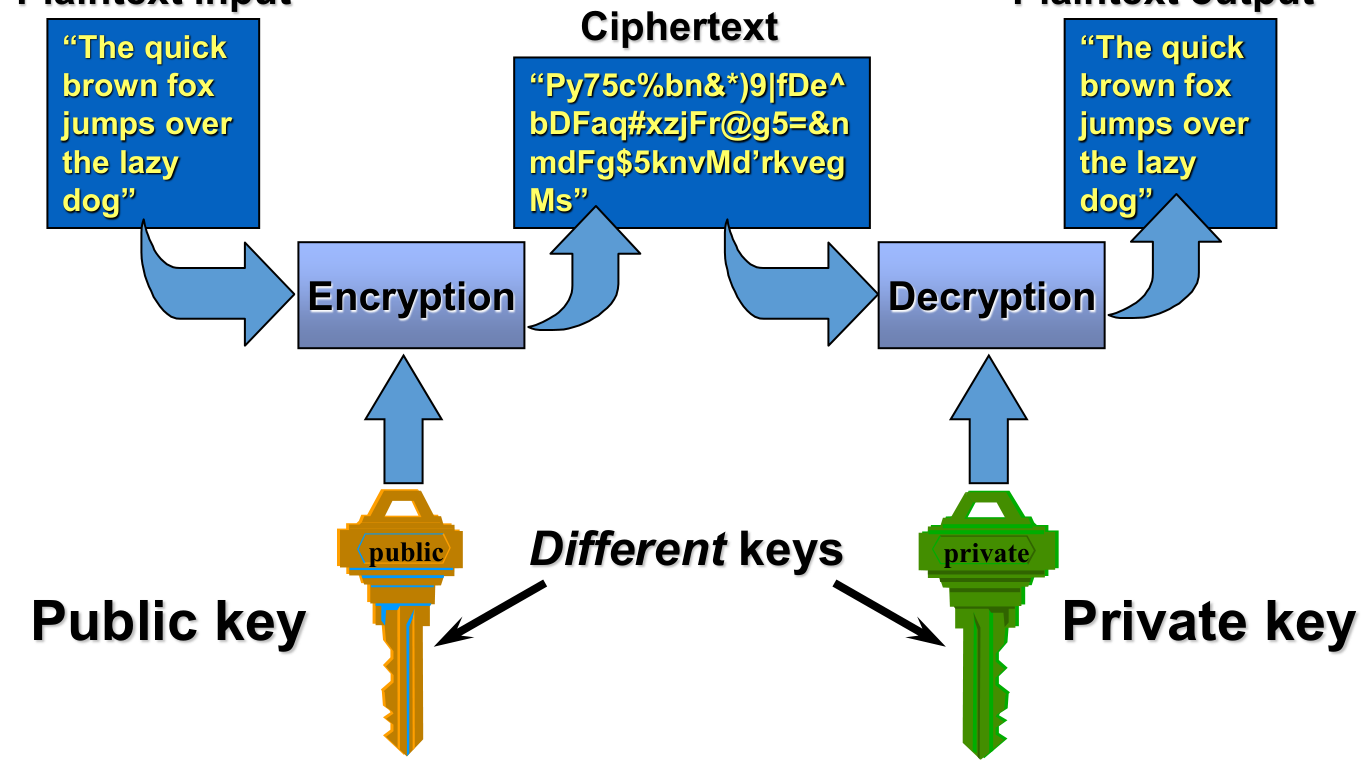
\includegraphics[width=149.10mm,height=210.87mm]{../../images/llm/page_061_img_01.png}%
\end{textblock*}

\end{document}
